\documentclass{beamer}

\usepackage[utf8]{inputenc}
\usepackage{epigraph}
\usepackage{tikz}
\usepackage{csquotes}
\usepackage{xcolor}
\usepackage{amssymb}
\usepackage{mdframed}
\usepackage{graphicx}
\usepackage{appendixnumberbeamer}
\usepackage{url}

\usetikzlibrary{patterns, arrows, cd, positioning, backgrounds, fit, decorations.pathmorphing, shapes.misc, calc, matrix, decorations.pathreplacing}
\tikzset{%
  node/.style={draw, minimum size=12mm, inner sep=0mm, circle, fill=gray!50},
  edge/.style={thick},
  move/.style={->},
  brace/.style={
    decorate,
    decoration={brace,amplitude=10pt,mirror},
  },
  table nodes/.style={
    rectangle,
    draw=black,
    align=center,
    minimum height=7mm,
    text depth=0.5ex,
    text height=2ex,
    inner xsep=0pt,
    outer sep=0pt
  },
  table/.style={
    matrix of nodes,
    row sep=\pgflinewidth,
    column sep=\pgflinewidth,
    nodes={
      table nodes
    }
  }
}



\usetheme{metropolis}
\metroset{numbering=fraction}
\setbeamercolor{math text}{fg=blue}

\DeclareMathOperator{\din}{\delta_{\mathit{in}}}
\DeclareMathOperator{\dout}{\delta_{\mathit{out}}}
\DeclareMathOperator{\Tid}{T_{\text{id}}}
\DeclareMathOperator{\Tsteps}{T_{\text{steps}}}
\DeclareMathOperator{\Twalk}{T_{\text{walk}}}
\DeclareMathOperator{\Thead}{T_{\text{head}}}

\title{Undirected Graph Exploration with $\Theta(\log\log n)$ Pebbles}
\subtitle{A Grimm idea}
\author{Christoph Welzel}
\institute{Logik und Theorie diskreter Systeme, RWTH Aachen}

\begin{document}
\maketitle
\begin{frame}
  \begin{center}
    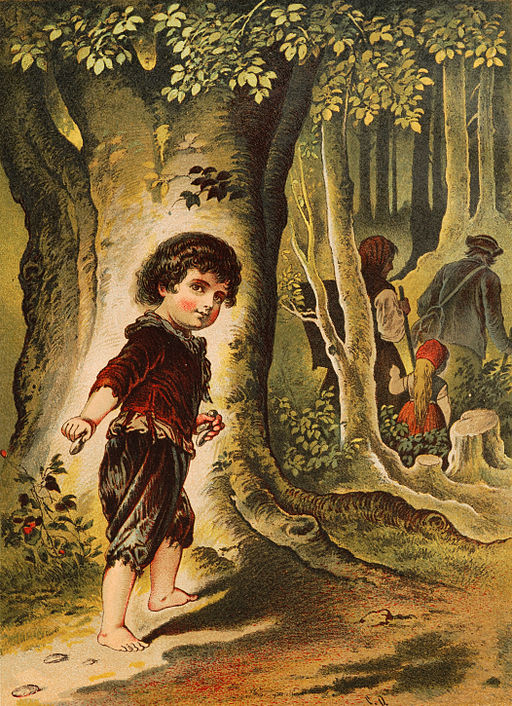
\includegraphics{hanselgretel.jpg}
  \end{center}
\end{frame}

\begin{frame}
  \frametitle{Introduction}
  \begin{itemize}
    \item Exploration of huge finite graphs by agents
    \item Agents are located on a vertex and move along edges
    \item Agents can drop pebbles on vertices
    \item Agent \emph{explores} a graph by systematically visiting all of
      its vertices
  \end{itemize}
\end{frame}

\section{Preliminaries}
\begin{frame}
  \frametitle{Huge graphs}
  \begin{columns}
    \column{0.55\textwidth}
    \begin{itemize}
      \item Undirected
      \item Finite, but huge
      \item Indistinguishable vertices:
      \parbox{\baselineskip}{
        \resizebox{!}{\baselineskip}{
          \begin{tikzpicture}
            \node[node] {};
          \end{tikzpicture}
        }
      }
      \item Bounded degree ($\Delta$)
      \item Edges can locally be labeled with
        \textcolor{blue}{$0,\dots,\Delta-1$} (Port)
    \end{itemize}
    \column{0.5\textwidth}
    \begin{center}
      \resizebox{\textwidth}{!}{\begin{tikzpicture}
  \node[node] (m1) {$v_{1}$};
  \node[node,right=2cm of m1] (m2) {$v_{2}$};

  \node[above left=of m1] (e1) {};
  \node[below=of m1] (e2) {};

  \node[above right=of m2] (e3) {};
  \node[below=of m2] (e4) {};

  \draw[edge] (m1) to node[very near start, above] {0} (e1);
  \draw[edge] (m1) to node[near start, left] {2} (e2);

  \draw[edge] (m2) to node[very near start, above] {1} (e3);
  \draw[edge] (m2) to node[near start, right] {2} (e4);
  
  \draw[edge] (m1) to node[very near start, below] {1} node[very near end, above] {0} (m2);
\end{tikzpicture}
}
    \end{center}
  \end{columns}
\end{frame}

\begin{frame}
  \frametitle{Agents}
  \begin{columns}
    \column{0.5\textwidth}
    \begin{itemize}
      \item Agent carries set of distinguishable pebbles
      \item Formalisation as pebble machines
        \begin{itemize}
          \item $(Q,F,P,m,\delta,\din,\dout,q_{0})$
          \item $(s,p,m)$-pebble machine
          \item<2-> $\din$: moving onto vertex
          \item<8-> $\dout$: leaving vertex
        \end{itemize}
    \end{itemize}
    \column{0.5\textwidth}
    \begin{itemize}
      \item<3-> As an agent moves onto a vertex it observes:
        \begin{itemize}
          \item<4-> Port it entered through
          \item<5-> Pebbles it carries
          \item<6-> Pebbles on the vertex
          \item<7-> Degree of vertex
        \end{itemize}
      \item<9-> Computation on a vertex determines:
        \begin{itemize}
          \item<10-> Port to leave
          \item<11-> Pebbles to drop
          \item<12-> Pebbles to carry along
        \end{itemize}
    \end{itemize}
  \end{columns}
\end{frame}


\begin{frame}
  \frametitle{Exploration sequence}
  \begin{columns}
    \column{0.6\textwidth}
    \begin{itemize}
      \item Exploration sequence $e_{1},\dots, e_{n}$
      \item Relative movements of agent
      \item Leaving port: $\ell_{i} + e_{i}\mod d_{v}$
      \item \emph{Universal} for a class of graphs if it explores any graph of
        that class
      \item<2->[$\rightarrow$] Example:
        $\alt<3-3>{\colorbox{green}{0}}{\colorbox{white!0}{0}},
        \alt<4-4>{\colorbox{green}{3}}{\colorbox{white!0}{3}},
        \alt<5-5>{\colorbox{green}{1}}{\colorbox{white!0}{1}},
        \alt<6-6>{\colorbox{green}{2}}{\colorbox{white!0}{2}}$
    \end{itemize}
    \column{0.4\textwidth}
    \begin{center}
      \resizebox{\textwidth}{!}{\begin{tikzpicture}
  \node[minimum size=12mm,inner sep=0mm, circle] (8) {};
  \node[node,right=of 8] (6) {};
  \node[node,right=of 6] (7) {};
  \node[node,below=of 8] (0) {};
  \node[node,below=of 6] (1) {};
  \node[node,below=of 7] (2) {};
  \node[node,below=of 0] (3) {};
  \node[node,below=of 1] (4) {};
  \node[node,below=of 2] (5) {};
  \node[node,above right=0.5cm and 1cm of 2] (8) {};
  \node[node,below right=0.5cm and 1cm of 2] (9) {};

  \draw[edge] (0) to node[very near start, above] {0} node[very near end, above] {1} (1);
  \draw[edge] (1) to node[very near start, below] {0} node[very near end, above] {1} (2);
  \draw[edge,bend right] (2.north west) to node[very near start, right] {0} node[very near end, above] {2} (0);
  \draw[edge] (0) to node[very near start, right] {1} node[very near end, left ] {0} (3);
  \draw[edge] (3) to node[very near start, above] {1} node[very near end, below] {1} (4);
  \draw[edge] (4) to node[very near start, below] {0} node[very near end, below] {1} (5);
  \draw[edge] (5) to node[very near start, above] {0} node[very near end, below] {2} (1);
  \draw[edge] (1) to node[very near start, left ] {3} node[very near end, left ] {2} (6);
  \draw[edge] (6) to node[very near start, above] {0} node[very near end, above] {1} (7);
  \draw[edge] (8) to node[very near start, above] {0} node[very near end, right] {0} (7);
  \draw[edge] (8) to node[very near start, above] {1} node[very near end, right] {2} (5);
  \draw[edge] (9) to node[very near start, below] {1} node[very near end, below] {3} (5);
  \draw[edge,bend right=20] (9) to node[very near start, below] {0} node[very near end, below] {1} (6);

  \begin{scope}[on background layer]%
      \node [fit=(0)] (layer) {};%
  \end{scope}
  \begin{scope}[on background layer]%
      \node [fit=(4)] (layer) {};%
  \end{scope}
  \only<3-3>{\begin{scope}[on background layer]%
      \node [fit=(0), fill=green!50] (layer) {};%
  \end{scope}}
  \only<4-4>{\begin{scope}[on background layer]%
      \node [fit=(3), fill=green!50] (layer) {};%
  \end{scope}}
  \only<5-5>{\begin{scope}[on background layer]%
      \node [fit=(4), fill=green!50] (layer) {};%
  \end{scope}}
  \only<6-6>{\begin{scope}[on background layer]%
      \node [fit=(3), fill=green!50] (layer) {};%
  \end{scope}}
  \only<7-7>{\begin{scope}[on background layer]%
      \node [fit=(4), fill=green!50] (layer) {};%
  \end{scope}}


\end{tikzpicture}
}
    \end{center}
  \end{columns}
\end{frame}

\section{Graph traversal}
\begin{frame}
  \frametitle{Exploring pebble machine}
  \begin{mdframed}
    \begin{theorem}[Reingold]
      There is an $\mathcal{O}(\log n)$-space algorithm producing a universal
      exploration sequence for any regular graph on $n$ vertices.
    \end{theorem}
  \end{mdframed}
  \begin{center}
    \begin{tikzpicture}
      \node (d1) {};
      \node[below=2 of d1] (d2) {};
      \draw[->, bend right] (d1) to (d2);
      \uncover<2->{
        \node[rectangle, draw=purple, below right=0.3 and 1 of d1]
        {3-Regularity};
      }
      \uncover<3->{
        \node[rectangle, draw=blue, below right=1 and 1.2 of d1]
        {Periodic Universal Lemma};
      }
      \uncover<4->{
        \node[rectangle, draw=magenta, below right=1.7 and 1 of d1]
        {Closed Walk Lemma};
      }
    \end{tikzpicture}
  \end{center}
  \begin{mdframed}
    \begin{theorem}
      There exists a $(\mathcal{O}(1), 0, \mathcal{O}(\log n))$-pebble machine
      that moves along a closed walk and either explores the graph or visits at
      least $n$ distinct vertices, for any graph with bounded degree.
    \end{theorem}
  \end{mdframed}
\end{frame}

\begin{frame}
  \frametitle{Closed walk}
  \begin{mdframed}[linecolor=magenta]
    \begin{lemma}[Closed Walk Lemma]
      An agent following an exploration sequence of the form
      $(e_{0},\dots,e_{k-1})^{\ast}$ moves along a closed walk.
    \end{lemma}
  \end{mdframed}
  \uncover<2->{
    \begin{mdframed}[linecolor=blue]
      \begin{lemma}[Periodic Universal Lemma]
        There exists an $\mathcal{O}(\log n)$-space algorithm producing a
        universal exploration sequence $(e_{0},\dots,e_{k-1})^{\ast}$ for any
        $3$-regular graph with at most $n$ vertices.
      \end{lemma}
    \end{mdframed}
  }
\end{frame}

\begin{frame}
  \frametitle{$3$-Regularity}
  \begin{mdframed}[linecolor=purple]
    Establish $3$-Regularity
  \end{mdframed}
  \begin{center}
    \uncover<2->{\resizebox{0.7\textwidth}{!}{\begin{tikzpicture}
  \node[node] (m1) {};
  \node[node] (m2) [right = 4cm of m1] {};
  \node[node] (m3) [right = 4cm of m2] {};

  \draw[edge] (m1) to node[below,very near start] {0} node[above,very near end] {1} (m2);
  \draw[edge] (m2) to node[above,very near start] {0} node[below,very near end] {0} (m3);

  \begin{scope}[on background layer]
    \node[fit=(m1),fill=green!50] (cl1) {};
    \node[fit=(m2),fill=yellow!50] (cl2) {};
    \node[fit=(m3),fill=red!50] (cl3) {};
  \end{scope}

  \uncover<3->{
    \node[node] (r11) [below = 6cm of m1] {0};
    \node[node] (r12) [above = 2cm of r11] {1};
    \node[node] (r13) [below = 2cm of r11] {2};

    \node[node] (l11) [below = 6cm of m3] {0};
    \node[node] (l12) [above = 2cm of l11] {1};
    \node[node] (l13) [below = 2cm of l11] {2};

    \node       (anker) [below = 6.5cm of m2] {};
    \node[node] (mid0) [above right = 1cm and 1cm of anker] {0};
    \node[node] (mid1) [below right = 1cm and 1cm of anker] {1};
    \node[node] (mid2) [below = 3cm of anker] {2};
    \node[node] (mid3) [below left = 1cm and 1cm of anker] {3};
    \node[node] (mid4) [above left = 1cm and 1cm of anker] {4};
    \node[node] (mid5) [above = 3cm of anker] {5};

    \draw[edge] (r11) to node[left,near end] {1} node[right,near start] {0} (r12);
    \draw[edge] (r11) to node[left,near end] {0} node[right,near start] {1} (r13);
    \draw[edge,bend right] (r12.south west) to node[left,very near end] {1} node[left, very near start] {0} (r13.north west);

    \draw[edge] (l11) to node[left,near end] {1} node[right,near start] {0}(l12);
    \draw[edge] (l11) to node[left,near end] {0} node[right,near start] {1}(l13);
    \draw[edge,bend left] (l12.south east) to node[left,very near end] {1} node[left, very near start] {0} (l13.north east);

    \draw[edge] (mid0) to node[right,near start] {0} node[right,near end] {1} (mid1);
    \draw[edge] (mid1) to node[right,near start] {0} node[right,near end] {1} (mid2);
    \draw[edge] (mid2) to node[left,near start] {0} node[left,near end] {1} (mid3);
    \draw[edge] (mid3) to node[left,near start] {0} node[left,near end] {1} (mid4);
    \draw[edge] (mid4) to node[left,near start] {0} node[left,near end] {1} (mid5);
    \draw[edge] (mid5) to node[right,near start] {0} node[right,near end] {1} (mid0);

    \draw[edge] (mid0) to node[very near start, above] {2} node[very near end, above] {2} (l11);
    \draw[edge] (mid2) to node[very near start, above] {2} node[very near end, above] {2} (l13);
    \draw[edge,bend left=10] (mid4) to node[very near start, below] {2} node[very near end, above] {2} (l12);

    \draw[edge] (mid1) to node[very near start, above] {2} node[very near end, above] {2} (r11);
    \draw[edge] (mid3) to node[very near start, above] {2} node[very near end, above] {2} (r13);
    \draw[edge] (mid5) to node[very near start, below] {2} node[very near end, above] {2} (r12);

    \only<3>{
      \begin{scope}[on background layer]
        \node[fit=(r11) (r12) (r13),fill=green!50] (cl1b) {};
        \node[fit=(mid0) (mid1) (mid2) (mid3) (mid4) (mid5),fill=yellow!50] (cl2b) {};
        \node[fit=(l11) (l12) (l13),fill=red!50] (cl3b) {};
        \draw[draw=green!50] (cl1.south west) to (cl1b.north west);
        \draw[draw=green!50] (cl1.south east) to (cl1b.north east);
        \draw[draw=yellow!50] (cl2.south west) to (cl2b.north west);
        \draw[draw=yellow!50] (cl2.south east) to (cl2b.north east);
        \draw[draw=red!50] (cl3.south west) to (cl3b.north west);
        \draw[draw=red!50] (cl3.south east) to (cl3b.north east);
      \end{scope}
    }
  }

\end{tikzpicture}
}}
  \end{center}
\end{frame}

\begin{frame}
  \frametitle{Exploring pebble machine}
  \begin{mdframed}
    \begin{theorem}[Reingold]
      There is an $\mathcal{O}(\log n)$-space algorithm producing a universal
      exploration sequence for any regular graph on $n$ vertices.
    \end{theorem}
  \end{mdframed}
  \begin{center}
    \begin{tikzpicture}
      \node (d1) {};
      \node[below=2 of d1] (d2) {};
      \draw[->, bend right] (d1) to (d2);
      \node[rectangle, draw=purple, below right=0.3 and 1 of d1]
        {3-Regularity};
      \node[rectangle, draw=blue, below right=1 and 1.2 of d1]
        {Periodic Universal Lemma};
      \node[rectangle, draw=yellow, below right=1.7 and 1 of d1]
        {Closed Walk Lemma};
    \end{tikzpicture}
  \end{center}
  \begin{mdframed}
    \begin{theorem}
      There exists a $(\mathcal{O}(1), 0, \mathcal{O}(\log n))$-pebble machine
      that moves along a closed walk and either explores the graph or visits at
      least $n$ distinct vertices, for any graph with bounded degree.
    \end{theorem}
  \end{mdframed}
\end{frame}

\section{Pebble simulation}
\begin{frame}
  \begin{mdframed}
    \begin{theorem}
      There is a constant $c\in\mathbb{N}$, such that for any graph $G$
      with bounded degree and any $(s,p,2m)$-pebble machine $\mathcal{M}$,
      there exists a $(cs,p+c,m)$-pebble machine $\mathcal{M}'$ that simulates
      the walk of $\mathcal{M}$ or explores $G$.
    \end{theorem}
  \end{mdframed}
\end{frame}

\begin{frame}
  \frametitle{Tape simulation via pebbles}
  \begin{itemize}
    \item Simulate $m$ bits by pebbles:
      \begin{itemize}
        \item<3-> Separate into $m_{1}$ sized blocks
        \item<4-> Represent blocks by pebbles
          $p_{0},\dots,p_{\frac{m}{m_{1}}-1}$
      \end{itemize}
  \end{itemize}
  \uncover<2->{\begin{tikzpicture}
  \matrix (tape) [table, text width=7mm, name=tape]
    { 1 & 1 & 0 & 0 & 1 & 0 & 0 & 1 & 1 & 0 & 0 & 0 \\};

  \node[above=of tape-1-1.west] (s1) {};
  \node[below=of tape-1-1.west] (s2) {};

  \node[above=of tape-1-3.east] (s3) {};
  \node[below=of tape-1-3.east] (s4) {};

  \node[above=of tape-1-6.east] (s5) {};
  \node[below=of tape-1-6.east] (s6) {};

  \node[above=of tape-1-9.east] (s7) {};
  \node[below=of tape-1-9.east] (s8) {};

  \node[above=of tape-1-12.east] (s9) {};
  \node[below=of tape-1-12.east] (s10) {};

  \uncover<2-2>{\draw[brace] (tape-1-12.north east) -- node[yshift=6mm] {$m = 12$} (tape-1-1.north west);}
  \uncover<3->{\draw[brace] (s9.center) -- node[yshift=6mm] {$m = 12$} (s1.center);}

  \uncover<3->{
    \draw[dashed] (s1) to (s2);
    \draw[dashed] (s3) to (s4);
    \draw[dashed] (s5) to (s6);
    \draw[dashed] (s7) to (s8);
    \draw[dashed] (s9) to (s10);
  }

  \uncover<3-3>{
    \draw[brace] (tape-1-1.south west) -- node[yshift=-6mm] {$m_{1} = 3$} (tape-1-3.south east);

    \draw[brace] (tape-1-4.south west) -- node[yshift=-6mm] {$m_{1} = 3$} (tape-1-6.south east);

    \draw[brace] (tape-1-7.south west) -- node[yshift=-6mm] {$m_{1} = 3$} (tape-1-9.south east);

    \draw[brace] (tape-1-10.south west) -- node[yshift=-6mm] {$m_{1} = 3$} (tape-1-12.south east);
  }
  \uncover<4-4>{
    \draw[brace] (tape-1-1.south west) -- node[yshift=-6mm]  {$p_{0}$} (tape-1-3.south east);

    \draw[brace] (tape-1-4.south west) -- node[yshift=-6mm]  {$p_{1}$} (tape-1-6.south east);

    \draw[brace] (tape-1-7.south west) -- node[yshift=-6mm]  {$p_{2}$} (tape-1-9.south east);

    \draw[brace] (tape-1-10.south west) -- node[yshift=-6mm] {$p_{3}$} (tape-1-12.south east);
  }
\end{tikzpicture}
}
\end{frame}

\begin{frame}
  \frametitle{Tape simulation via pebbles}
  \begin{tikzpicture}
  \matrix (tape) [table, text width=7mm, name=tape]
    { 1 & 1 & 0 & 0 & 1 & 0 & 0 & 1 & 1 & 0 & 0 & 0 \\};
  \draw[brace] (tape-1-1.south west) -- node[yshift=-6mm] {$p_{0}$} (tape-1-3.south east); 
  \draw[brace] (tape-1-4.south west) -- node[yshift=-6mm] {$p_{1}$} (tape-1-6.south east); 
  \draw[brace] (tape-1-7.south west) -- node[yshift=-6mm] {$p_{2}$} (tape-1-9.south east); 
  \draw[brace] (tape-1-10.south west) -- node[yshift=-6mm] {$p_{3}$} (tape-1-12.south east); 
\end{tikzpicture}

  \begin{columns}
    \column{0.5\textwidth}
    \begin{itemize}
      \item Pebble needs $2^{m_{1}}$ distinct \enquote{states}
      \item State as index of closed walk
    \end{itemize}
    \column{0.5\textwidth}
    \resizebox{\textwidth}{!}{\begin{tikzpicture}
  \node[minimum size=12mm,inner sep=0mm, circle] (8) {};
  \node[node,right=of 8,label={100:$p_{0}$}] (6) {$6$};
  \node[node,right=of 6] (7) {$7$};
  \node[node,below=of 8,label={100:$p_{3}$}] (0) {$0$};
  \node[node,below=of 6] (1) {$1$};
  \node[node,below=of 7,label={$p_{1}$}] (2) {$2$};
  \node[node,below=of 0,label={45:$p_{2}$}] (3) {$3$};
  \node[node,below=of 1] (4) {$4$};
  \node[node,below=of 2] (5) {$5$};

  \draw[move] (0) to (1);
  \draw[move] (1) to (2);
  \draw[move,bend left] (2.south west) to (0);
  \draw[move] (0) to (3);
  \draw[move] (3) to (4);
  \draw[move] (4) to (5);
  \draw[move] (5) to (1);
  \draw[move] (1) to (6);
  \draw[move] (6) to (7);
  \draw[dashed, move, decorate,
  decoration={snake,amplitude=0.5cm, segment length=3cm}, bend right=55]
  (7.north west) to (0);
\end{tikzpicture}
}
  \end{columns}
\end{frame}

\begin{frame}
  \frametitle{Mechanisms of simulation}
  \begin{enumerate}
    \item Simulation of $M_{\text{walk}}$ providing
        walk with $2^{m_{1}}$ distinct vertices
    \item \textcolor<2->{blue}{Identify \emph{distinct} vertices of walk}
    \item Read from and write to simulated tape
    \item Preserve tape content through steps of simulated agent
  \end{enumerate}
\end{frame}


\begin{frame}
  \frametitle{2. Finding distinct vertices}
  Problem: Indistinguishable vertices $\leadsto$ next vertex \enquote{new}?
  \begin{columns}
    \column{0.5\textwidth}
    Solution:
    \begin{enumerate}
      \item \textcolor<3,8>{magenta}{Execute step of $M_{\text{walk}}$}
      \item \textcolor<4,9>{magenta}{Drop pebble $p_{\text{tmp}}$}
      \item \textcolor<4,9>{magenta}{Store number of steps $M_{\text{walk}}$
        executed}
      \item \textcolor<5,10>{magenta}{Restart $M_{\text{walk}}$}
      \item \textcolor<6,11-18>{magenta}{Execute steps of $M_{\text{walk}}$
          until $p_{\text{tmp}}$ is observed}
      \item \textcolor<19-20>{magenta}{Same amount of steps for
        $M_{\text{walk}}$ to find $p_{\text{tmp}}$ $\rightarrow$ new vertex}
      \item \textcolor<7>{magenta}{Otherwise start over}
    \end{enumerate}
    \column{0.5\textwidth}
    \begin{tikzpicture}
  \node[minimum size=12mm,inner sep=0mm, circle] (8) {};
  \node[node,right=of 8,label={100:$p_{0}$}] (6) {\only<20-20>{$6$}};
  \node[node,right=of 6] (7) {};
  \node[node,below=of 8,label={100:$p_{3}$}] (0) {$0$};
  \node[node,below=of 6] (1) {$1$};
  \node[node,below=of 7,label={$p_{1}$}] (2) {$2$};
  \node[node,below=of 0,label={45:$p_{2}$}] (3) {$3$};
  \node[node,below=of 1] (4) {$4$};
  \node[node,below=of 2] (5) {$5$};
  \node[fill=blue!50, above right=-0.1cm and -0.1cm of 0] (pstart) {$p_{\text{start}}$};

  \draw[move] (0) to (1);
  \draw[move] (1) to (2);
  \draw[move,bend left] (2.south west) to (0);
  \draw[move] (0) to (3);
  \draw[move] (3) to (4);
  \draw[move] (4) to (5);
  \draw[move] (5) to (1);
  \draw[move] (1) to (6);
  \draw[move] (6) to (7);
  \draw[dashed, move, decorate,
  decoration={snake,amplitude=0.5cm, segment length=3cm}, bend right=55]
  (7.north west) to (0);

  % placement dummies:
  \begin{scope}[on background layer]
    \node[fit=(5)] (d1) {};
  \end{scope}
  \begin{scope}[on background layer]
    \node[fit=(4)] (d2) {};
  \end{scope}
  \begin{scope}[on background layer]
    \node[fit=(3)] (d3) {};
  \end{scope}
  \begin{scope}[on background layer]
    \node[fit=(2)] (d4) {};
  \end{scope}
  \begin{scope}[on background layer]
    \node[fit=(1)] (d5) {};
  \end{scope}
  \begin{scope}[on background layer]
    \node[fit=(0)] (d6) {};
  \end{scope}

  \only<2-2>{
    \begin{scope}[on background layer]
      \node[fit=(5), fill=green!50] (s0) {};
    \end{scope}
  }
  \only<3-4>{
    \begin{scope}[on background layer]
      \node[fit=(1), fill=green!50] (s1) {};
    \end{scope}
  }
  \only<4-6>{
    \node[fill=blue!50, above right=-0.1cm and -0.1cm of 1] (ptmp1) {$p_{\text{tmp}}$};
  }
  \only<5-5>{
    \begin{scope}[on background layer]
      \node[fit=(0), fill=red!50] (s2) {};
    \end{scope}
  }
  \only<6-6>{
    \begin{scope}[on background layer]
      \node[fit=(1), fill=red!50] (s3) {};
    \end{scope}
  }
  \only<7-7>{
    \begin{scope}[on background layer]
      \node[fit=(1), fill=green!50] (s4) {};
    \end{scope}
  }
  \only<8-9>{
    \begin{scope}[on background layer]
      \node[fit=(6), fill=green!50] (s5) {};
    \end{scope}
  }
  \only<9-18>{
    \node[fill=blue!50, above right=-0.1cm and -0.1cm of 6] (ptmp2) {$p_{\text{tmp}}$};
  }
  \only<10-10>{
    \begin{scope}[on background layer]
      \node[fit=(0), fill=red!50] (s6) {};
    \end{scope}
  }
  \only<11-11>{
    \begin{scope}[on background layer]
      \node[fit=(1), fill=red!50] (s7) {};
    \end{scope}
  }
  \only<12-12>{
    \begin{scope}[on background layer]
      \node[fit=(2), fill=red!50] (s8) {};
    \end{scope}
  }
  \only<13-13>{
    \begin{scope}[on background layer]
      \node[fit=(0), fill=red!50] (s9) {};
    \end{scope}
  }
  \only<14-14>{
    \begin{scope}[on background layer]
      \node[fit=(3), fill=red!50] (s10) {};
    \end{scope}
  }
  \only<15-15>{
    \begin{scope}[on background layer]
      \node[fit=(4), fill=red!50] (s12) {};
    \end{scope}
  }
  \only<16-16>{
    \begin{scope}[on background layer]
      \node[fit=(5), fill=red!50] (s13) {};
    \end{scope}
  }
  \only<17-17>{
    \begin{scope}[on background layer]
      \node[fit=(1), fill=red!50] (s13) {};
    \end{scope}
  }
  \only<18-18>{
    \begin{scope}[on background layer]
      \node[fit=(6), fill=red!50] (s14) {};
    \end{scope}
  }
  \only<19-20>{
    \begin{scope}[on background layer]
      \node[fit=(6), fill=green!50] (s14) {};
    \end{scope}
  }
\end{tikzpicture}

  \end{columns}
\end{frame}



\begin{frame}
  \frametitle{Simulation of a pebble machine}
  \begin{itemize}
    \item Simulation of $M_{\text{Walk}}$ which explores at least $2^{m_{1}}$
      distinct vertices \uncover<2->{\textcolor{green}{{\checkmark}}}
    \item Identify \emph{distinct} vertices of the walk
      \uncover<3->{\textcolor{green}{{\checkmark}}}
    \item Read from and write to simulated tape \uncover<4->{\textcolor{green}{{\checkmark}}}
    \item Preserve tape content through steps of simulated agent
      \uncover<5->{\textcolor{green}{{\checkmark}}}
  \end{itemize}
  \uncover<6->{
    \begin{mdframed}
      \begin{theorem}
        There is a constant $c\in\mathbb{N}$, such that for any graph $G$
        with bounded degree and any $(s,p,2m)$-pebble machine $\mathcal{M}$,
        there exists a $(cs,p+c,m)$-pebble machine $\mathcal{M}'$ that simulates
        the walk of $\mathcal{M}$ or explores $G$.
      \end{theorem}
    \end{mdframed}
  }
\end{frame}

\begin{frame}
  \frametitle{Exploring graphs with $\log\log n$ pebbles}
  \begin{mdframed}
    \begin{theorem}
      There exists a $(\mathcal{O}(1), 0, \mathcal{O}(\log n))$-pebble machine
      that moves along a closed walk and either explores the graph or visits at
      least $n$ distinct vertices, for any graph with bounded degree.
    \end{theorem}
  \end{mdframed}
  \begin{center}
    \begin{tikzpicture}
      \node (d1) {};
      \node[below=1.5 of d1] (d2) {};
      \draw[->, bend right] (d1) to (d2);
      \node[below right=0.6 and 1 of d1, rectangle,draw=black] {Apply simulation Theorem $\log\log n$ times};
    \end{tikzpicture}
  \end{center}
  \begin{mdframed}
    \begin{theorem}
      Any bounded-degree graph on at most $n$ vertices can be explored using
      $\mathcal{O}(\log\log n)$ pebbles and memory.
    \end{theorem}
  \end{mdframed}
\end{frame}

\section{Limitations of pebble machines}
\begin{frame}
  \frametitle{Limitations of pebbles}
  \begin{itemize}
    \item Construct $3$-regular graphs which an agent $\mathcal{A}$ with $p$
      pebbles cannot traverse
    \item Called $p$-barriers
      \begin{center}
        \resizebox{0.6\textwidth}{!}{\begin{tikzpicture}
\node[node] (v1) {$v_{1}$};
\node[node, below=of v1] (v2) {$v_{2}$};

\node[node, right=of v1] (v3) {$v_{3}$};
\node[node, below=of v3] (v4) {$v_{4}$};

\node[fit=(v1) (v2) (v3) (v4), draw=black] (b) {};
\draw[dashed, thick] (b.north) to (b.south);

\only<1>{
  \draw[edge] (v1) to (v2);
  \draw[edge] (v3) to (v4);
}

\uncover<2>{
  \node[left=3 of v1] (d1) {};
  \node[left=2 of d1] (d3) {};
  \node[left=3 of v2] (d2) {};
  \node[left=2 of d2] (d4) {};
  \node[fit=(d1) (d2) (d3) (d4), draw=black, rectangle] (g) {};
  \node[below left=0.75 of d1] (G) {$G$};
  \draw[bend right] (v1) to (d1);
  \draw[bend right] (v3) to (d3);
  \draw[bend right] (v2) to (d2);
  \draw[bend right] (v4) to (d4);
}
\end{tikzpicture}
}
      \end{center}
    \item For every pair $(a,b)$ in
      $\left\{v_{1},v_{2}\right\}\times\left\{v_{3},v_{4}\right\}$
      $\mathcal{A}$ cannot traverse a $p$-barrier from $a$ to $b$
      or vice versa using at most $p$ pebbles
    \item Inductive construction of barriers
  \end{itemize}
\end{frame}

\begin{frame}
  \frametitle{Locality gadget}
  \begin{itemize}
    \item Replace edge by $(r-1)$-barrier
    \item Enforce \enquote{locality} of pebbles
      \begin{center}
        \uncover<2->{\resizebox{0.8\textwidth}{!}{\begin{tikzpicture}
  \node[node] (0) {$v$};
  \node[node,above right=of 0] (1) {};
  \node[node,above left=of 0] (2) {};
  \node[node,below=of 0] (3) {};

  \draw[edge] (0) to (1);
  \draw[edge] (0) to (2);
  \draw[edge] (0) to (3);

  \node[node,right=5cm of 0] (0') {$v$};
  \node[node,above right=of 0'] (1') {};
  \node[node,above left=of 0'] (2') {};
  \node[node,below=of 0'] (3') {};

  \draw[edge,on background layer] (0') to node[draw,midway,fill=gray,shape=rectangle] {$B$} (1');
  \draw[edge,on background layer] (0') to node[draw,midway,fill=gray,shape=rectangle] {$B$} (2');
  \draw[edge,on background layer] (0') to node[draw,midway,fill=gray,shape=rectangle] {$B$} (3');

  \draw[->, shorten <=0.2cm, shorten >=0.2cm,
  decorate,decoration={snake,amplitude=0.3cm, segment length=1.0cm}] (0) to (0');
\end{tikzpicture}
}}
      \end{center}
  \end{itemize}
\end{frame}

\begin{frame}
  \begin{mdframed}
    \begin{theorem}
      Given an $(r-1)$-barrier $B$ with $m$ vertices for an agent $\mathcal{A}$
      with $p\geq r$ pebbles, we can construct an $r$-barrier $B'$ with
      $\mathcal{O}(\binom{p}{r}\cdot m\cdot\alpha_{B}^{2})$ vertices for
      $\mathcal{A}$.
    \end{theorem}
  \end{mdframed}
  where $\alpha_{B}$ is the amount of \enquote{local} configurations for
  $\mathcal{A}$ with $r$ pebbles
\end{frame}

\begin{frame}
  \frametitle{Barrier construction: Idea}
  \begin{columns}
    \column{0.5\textwidth}
    \begin{itemize}
      \item Subset of pebbles of cardinality $r$
      \item Locality gadget as edges
      \item Pebbles are local: configurations in macro vertex
        $C_{1},\dots,C_{\alpha}$
      \item Project $A$ to agent without pebbles $B$
      \item $B$ has $\alpha$ states and traverses macro vertices
    \end{itemize}
    \column{0.5\textwidth}
    \resizebox{\textwidth}{!}{\begin{tikzpicture}
  \node[node] (a0) {$m_{0}$};
  \node[node,right=of a0] (a1) {$m_{1}$};

  \node[node,below=of a0] (b0) {$m_{0}$};
  \node[node,right=of b0] (b1) {$m_{1}$};

  \begin{scope}[on background layer]
    \node[fit=(a0)] (dummy1) {};
    \node[fit=(a1)] (dummy2) {};
    \node[fit=(b0)] (dummy3) {};
    \node[fit=(b1)] (dummy4) {};
  \end{scope}

  \node[rectangle,fill=gray!50, right=0.25 of a0] (b) {$B$};

  \draw[edge] (a0) to (b);
  \draw[edge] (b) to (a1);
  \draw[edge] (b0) to (b1);

  \only<1-1> {
    \begin{scope}[on background layer]
      \node[fit=(a0),fill=green!50] {};
      \node[fit=(b0),fill=blue!50] {};
    \end{scope}
  }
  \only<2-2> {
    \begin{scope}[on background layer]
      \node[fit=(b),fill=green!50] {};
      \node[fit=(b1),fill=blue!50] {};
    \end{scope}
  }
  \only<3-3> {
    \begin{scope}[on background layer]
      \node[fit=(a1),fill=green!50] {};
      \node[fit=(b1),fill=blue!50] {};
    \end{scope}
  }
\end{tikzpicture}
}
  \end{columns}
\end{frame}

\begin{frame}
  \frametitle{Barrier construction}
  \begin{itemize}
    \item $B$ has no pebbles and cannot traverse $0$-barrier
    \item $r$-barrier for chosen subset of pebbles
    \item Connect barriers for all possible subsets of pebbles with cardinality
      $r$:
  \end{itemize}
  \begin{center}
    \resizebox{0.8\textwidth}{!}{\begin{tikzpicture}
  \node[node] (b0l0) {};
  \node[node,below=2 of b0l0] (b0l1) {};
  \node[node,right=of b0l0] (b0r0) {};
  \node[node,below=2 of b0r0] (b0r1) {};
  \node[fit=(b0l0) (b0l1) (b0r0) (b0r1),draw=black,label={90:$H_{1}$}] (b0) {};
  \draw[dashed, thick] (b0.north) to (b0.south);

  \node[node,right=of b0r0] (b1l0) {};
  \node[node,below=2 of b1l0] (b1l1) {};
  \node[node,right=of b1l0] (b1r0) {};
  \node[node,below=2 of b1r0] (b1r1) {};
  \node[fit=(b1l0) (b1l1) (b1r0) (b1r1),draw=black,label={90:$H_{2}$}] (b1) {};
  \draw[dashed, thick] (b1.north) to (b1.south);

  \node[minimum size=12mm,circle,right=of b1r0] (b2l0) {};
  \node[minimum size=12mm,circle,below=2 of b2l0] (b2l1) {};
  \node[minimum size=12mm,circle,right=of b2l0] (b2r0) {};
  \node[minimum size=12mm,circle,below=2 of b2r0] (b2r1) {};

  \node[node,right=of b2r0] (b3l0) {};
  \node[node,below=2 of b3l0] (b3l1) {};
  \node[node,right=of b3l0] (b3r0) {};
  \node[node,below=2 of b3r0] (b3r1) {};
  \node[fit=(b3l0) (b3l1) (b3r0) (b3r1),draw=black,label={90:$H_{{n}\choose{p}}$}] (b2) {};
  \draw[dashed, thick] (b1.north) to (b1.south);

  \draw[edge] (b0r0) to (b1l0);
  \draw[edge] (b0r1) to (b1l1);
  \draw[dashed] (b1r0) to (b2l0);
  \draw[dashed] (b1r1) to (b2l1);
  \draw[dashed] (b2r0) to (b3l0);
  \draw[dashed] (b2r1) to (b3l1);

  \draw[edge] (b0l0) to (b0l1);
  \draw[edge] (b3r0) to (b3r1);

  \node[fit=(b0) (b1) (b2), draw=black, label={90:$B$},inner sep=12mm] (b) {};
\end{tikzpicture}
}
  \end{center}
\end{frame}

\begin{frame}
  \frametitle{Barrier base case}
  \begin{mdframed}
    \begin{theorem}[Fraigniaud et al.]
      For any $q$ non cooperative $s$-state agents without pebbles, there
      exists a $3$-regular graph $G$ on $\mathcal{O}(qs)$ vertices with the
      following property: There are two edges $\left\{v_{1},v_{2}\right\}$
      and $\left\{v_{3},v_{4}\right\}$ in $G$, the first labeled 0, such
      that any of the $q$ agents starting in $v_{1}$ or $v_{2}$ does not
      traverse the edge $\left\{v_{3},v_{4}\right\}$.
    \end{theorem}
  \end{mdframed}
  \begin{itemize}
    \item For agent $\mathcal{A}$ consider
      $S = \left\{\mathcal{A}_{q}\mid q\in Q\right\}$
    \item Since $|S| = |Q| = q$ there is a 0-barrier with $\mathcal{O}(s^{2})$
      vertices
  \end{itemize}
\end{frame}

\begin{frame}
  \frametitle{Barrier}
  \begin{mdframed}
    \begin{theorem}
      Given an $(r-1)$-barrier $B$ with $m$ vertices for an agent $\mathcal{A}$
      with $p\geq r$ pebbles, we can construct an $r$-barrier $B'$ with
      $\mathcal{O}(\binom{p}{r}\cdot m\cdot\alpha_{B}^{2})$ vertices for
      $\mathcal{A}$.
    \end{theorem}
  \end{mdframed}
  \begin{center}
    \resizebox{0.7\textwidth}{!}{\begin{tikzpicture}
  \node[node] (b0l0) {};
  \node[node,below=2 of b0l0] (b0l1) {};
  \node[node,right=of b0l0] (b0r0) {};
  \node[node,below=2 of b0r0] (b0r1) {};
  \node[fit=(b0l0) (b0l1) (b0r0) (b0r1),draw=black,label={90:$H_{1}$}] (b0) {};
  \draw[dashed, thick] (b0.north) to (b0.south);

  \node[node,right=of b0r0] (b1l0) {};
  \node[node,below=2 of b1l0] (b1l1) {};
  \node[node,right=of b1l0] (b1r0) {};
  \node[node,below=2 of b1r0] (b1r1) {};
  \node[fit=(b1l0) (b1l1) (b1r0) (b1r1),draw=black,label={90:$H_{2}$}] (b1) {};
  \draw[dashed, thick] (b1.north) to (b1.south);

  \node[minimum size=12mm,circle,right=of b1r0] (b2l0) {};
  \node[minimum size=12mm,circle,below=2 of b2l0] (b2l1) {};
  \node[minimum size=12mm,circle,right=of b2l0] (b2r0) {};
  \node[minimum size=12mm,circle,below=2 of b2r0] (b2r1) {};

  \node[node,right=of b2r0] (b3l0) {};
  \node[node,below=2 of b3l0] (b3l1) {};
  \node[node,right=of b3l0] (b3r0) {};
  \node[node,below=2 of b3r0] (b3r1) {};
  \node[fit=(b3l0) (b3l1) (b3r0) (b3r1),draw=black,label={90:$H_{{n}\choose{p}}$}] (b2) {};
  \draw[dashed, thick] (b1.north) to (b1.south);

  \draw[edge] (b0r0) to (b1l0);
  \draw[edge] (b0r1) to (b1l1);
  \draw[dashed] (b1r0) to (b2l0);
  \draw[dashed] (b1r1) to (b2l1);
  \draw[dashed] (b2r0) to (b3l0);
  \draw[dashed] (b2r1) to (b3l1);

  \draw[edge] (b0l0) to (b0l1);
  \draw[edge] (b3r0) to (b3r1);

  \node[fit=(b0) (b1) (b2), draw=black, label={90:$B$},inner sep=12mm] (b) {};
\end{tikzpicture}
}
  \end{center}
\end{frame}


\begin{frame}
  \frametitle{Lower pebble bound}
  \begin{mdframed}
    \begin{theorem}
      For $r\leq p$ and $s\geq 2^{p}$, the number of vertices of an $r$-barrier
      $B_{r}$ for the $s$-state agent $\mathcal{A}$ with $p$ pebbles is bounded
      by $\mathcal{O}(s^{8^{r+1}})$.
    \end{theorem}
  \end{mdframed}
  \begin{center}
    \begin{tikzpicture}
      \node (d1) {};
      \node[below=1.5 of d1] (d2) {};
      \draw[->, bend right] (d1) to (d2);
    \end{tikzpicture}
  \end{center}
  \begin{mdframed}
    \begin{theorem}
      For any constant $\epsilon > 0$, an agent with at most
      $\mathcal{O}((\log n)^{1-\epsilon})$ bits of memory needs at least
      $\Omega(\log\log n)$ distinguishable pebbles for exploring all
      graphs on at most $n$ vertices.
    \end{theorem}
  \end{mdframed}
\end{frame}

\section{Conclusion}
\begin{frame}
  \frametitle{Conclusion}
  \begin{itemize}
    \item Exploring graphs with $\mathcal{O}(\log\log n)$ pebbles and memory
    \item Simulation via pebbles
    \item Limitations of pebbles: Barrier construction
    \item Every agent with sub-logarithmic memory needs $\Omega(\log\log n)$
      pebbles to explore $n$ vertices
  \end{itemize}
\end{frame}

\begin{frame}
  \vspace{0.3\textheight}
  \begin{center}
    {\Huge Thank you for your attention.}
  \end{center}
  \vspace{0.35\textheight}
  Slides and report on \url{https://github.com/weltoph/sem-pebbles}.
\end{frame}

\appendix
\begin{frame}
  \frametitle{1. Simulation of $M_{\text{walk}}$}
  \begin{itemize}
    \item $M_{\text{Walk}}$ implemented as
      $(\mathcal{O}(1), 0, \mathcal{O}(m_{1}))$-pebble machine
    \item Used variables/pebbles:
      \begin{itemize}
        \item $\Twalk$: stores $M_{\text{walk}}$'s tape
        \item $\Tsteps$: stores number of taken steps
        \item $\Tid$: stores number of visited distinct vertices
        \item $p_{\text{start}}$: marks beginning of walk
      \end{itemize}
  \end{itemize}
\end{frame}

\begin{frame}
  \frametitle{3. Memory management}
  \begin{columns}
    \column{0.5\textwidth}
    \begin{itemize}
      \item $\Thead$: head position
      \item $p_{\left\lfloor\frac{\Thead}{m_{1}}\right\rfloor}$: pebble of
        memory block
      \item $\mathit{off} = \Thead\mod m_{1}$: offset in memory block
      \item Reading:
        \begin{itemize}
          \item Retrieve encoding pebble
          \item Return $\mathit{off}$-th bit
        \end{itemize}
      \item Writing:
        \begin{itemize}
          \item Read bit
          \item On bit-flip move encoding pebble $2^{\mathit{off}}$ bits up or
            down
        \end{itemize}
    \end{itemize}
    \column{0.5\textwidth}
    \resizebox{\textwidth}{!}{\begin{tikzpicture}
  \matrix (tape) [table, text width=7mm, name=tape]
    { 1 & 1 & 0 & 0 & 1 & 0 & 0 & 1 & 1 & 0 & 0 & 0 \\};
  \draw[brace] (tape-1-1.south west) -- node[yshift=-6mm] {$p_{0}$} (tape-1-3.south east); 
  \draw[brace] (tape-1-4.south west) -- node[yshift=-6mm] {$p_{1}$} (tape-1-6.south east); 
  \draw[brace] (tape-1-7.south west) -- node[yshift=-6mm] {$p_{2}$} (tape-1-9.south east); 
  \draw[brace] (tape-1-10.south west) -- node[yshift=-6mm] {$p_{3}$} (tape-1-12.south east); 
\end{tikzpicture}
}
    \resizebox{\textwidth}{!}{\begin{tikzpicture}
  \node[minimum size=12mm,inner sep=0mm, circle] (8) {};
  \node[node,right=of 8,label={100:$p_{0}$}] (6) {$6$};
  \node[node,right=of 6] (7) {$7$};
  \node[node,below=of 8,label={100:$p_{3}$}] (0) {$0$};
  \node[node,below=of 6] (1) {$1$};
  \node[node,below=of 7,label={$p_{1}$}] (2) {$2$};
  \node[node,below=of 0,label={45:$p_{2}$}] (3) {$3$};
  \node[node,below=of 1] (4) {$4$};
  \node[node,below=of 2] (5) {$5$};

  \draw[move] (0) to (1);
  \draw[move] (1) to (2);
  \draw[move,bend left] (2.south west) to (0);
  \draw[move] (0) to (3);
  \draw[move] (3) to (4);
  \draw[move] (4) to (5);
  \draw[move] (5) to (1);
  \draw[move] (1) to (6);
  \draw[move] (6) to (7);
  \draw[dashed, move, decorate,
  decoration={snake,amplitude=0.5cm, segment length=3cm}, bend right=55]
  (7.north west) to (0);
\end{tikzpicture}
}
  \end{columns}
\end{frame}

\begin{frame}
  \frametitle{3. Memory management: Writing}
  \begin{itemize}
    \item Read bit
    \item On bit-flip: move pebble
  \end{itemize}
  \resizebox{\textwidth}{!}{\begin{tikzpicture}
  \node[minimum size=12mm,inner sep=0mm, circle] (8) {};
  \node[node,right=of 8,label={100:\alt<0-11>{$p_{0}$}{}}] (6) {$6$};
  \node[node,right=of 6] (7) {$7$};
  \node[node,below=of 8,label={100:$p_{3}$}] (0) {$0$};
  \node[node,below=of 6] (1) {$1$};
  \node[node,below=of 7,label={$p_{1}$}] (2) {$2$};
  \node[node,below=of 0,label={45:$p_{2}$}] (3) {$3$};
  \node[node,below=of 1,label={90:\alt<0-19>{}{$p_{0}$}}] (4) {$4$};
  \node[node,below=of 2] (5) {$5$};

  \draw[move] (0) to (1);
  \draw[move] (1) to (2);
  \draw[move,bend left] (2.south west) to (0);
  \draw[move] (0) to (3);
  \draw[move] (3) to (4);
  \draw[move] (4) to (5);
  \draw[move] (5) to (1);
  \draw[move] (1) to (6);
  \draw[move] (6) to (7);
  \draw[dashed, move, decorate,
  decoration={snake,amplitude=0.5cm, segment length=3cm}, bend right=55]
  (7.north west) to (0);

  \matrix (tape) [left=of 0, table, text width=7mm, name=tape]
    { 1 & \alt<0-12>{1}{0} & 0 & 0 & 1 & 0 & 0 & 1 & 1 & 0 & 0 & 0 \\};
  \draw[brace] (tape-1-1.south west) -- node[yshift=-6mm] {$p_{0}$} (tape-1-3.south east); 
  \draw[brace] (tape-1-4.south west) -- node[yshift=-6mm] {$p_{1}$} (tape-1-6.south east); 
  \draw[brace] (tape-1-7.south west) -- node[yshift=-6mm] {$p_{2}$} (tape-1-9.south east); 
  \draw[brace] (tape-1-10.south west) -- node[yshift=-6mm] {$p_{3}$} (tape-1-12.south east); 

  \begin{scope}[on background layer]
    \node[fit=(0)] (d0) {};
  \end{scope}
  \begin{scope}[on background layer]
    \node[fit=(1)] (d1) {};
  \end{scope}
  \begin{scope}[on background layer]
    \node[fit=(2)] (d2) {};
  \end{scope}
  \begin{scope}[on background layer]
    \node[fit=(3)] (d3) {};
  \end{scope}
  \begin{scope}[on background layer]
    \node[fit=(4)] (d4) {};
  \end{scope}
  \begin{scope}[on background layer]
    \node[fit=(5)] (d5) {};
  \end{scope}
  \begin{scope}[on background layer]
    \node[fit=(6)] (d6) {};
  \end{scope}
  \begin{scope}[on background layer]
    \node[fit=(7)] (d7) {};
  \end{scope}

  \uncover<2->{
    \node[above right=0.6cm and 0.0cm of tape-1-2] (marker) {\alt<2-12>{0}{}};
    \draw[red, thick, ->] (marker) to (tape-1-2.north);
  }
  \only<3-3>{
    \begin{scope}[on background layer]
      \node[fit=(0), fill=red!50] (s1) {};
    \end{scope}
  }
  \only<4-4>{
    \begin{scope}[on background layer]
      \node[fit=(1), fill=red!50] (s2) {};
    \end{scope}
  }
  \only<5-5>{
    \begin{scope}[on background layer]
      \node[fit=(2), fill=red!50] (s3) {};
    \end{scope}
  }
  \only<6-6>{
    \begin{scope}[on background layer]
      \node[fit=(0), fill=red!50] (s4) {};
    \end{scope}
  }
  \only<7-7>{
    \begin{scope}[on background layer]
      \node[fit=(3), fill=red!50] (s5) {};
    \end{scope}
  }
  \only<8-8>{
    \begin{scope}[on background layer]
      \node[fit=(4), fill=red!50] (s6) {};
    \end{scope}
  }
  \only<9-9>{
    \begin{scope}[on background layer]
      \node[fit=(5), fill=red!50] (s7) {};
    \end{scope}
  }
  \only<10-10>{
    \begin{scope}[on background layer]
      \node[fit=(1), fill=red!50] (s8) {};
    \end{scope}
  }
  \only<11-11>{
    \begin{scope}[on background layer]
      \node[fit=(6), fill=red!50] (s9) {};
    \end{scope}
  }
  \only<14-14>{
    \begin{scope}[on background layer]
      \node[fit=(0), fill=red!50] (s10) {};
    \end{scope}
  }
  \only<15-15>{
    \begin{scope}[on background layer]
      \node[fit=(1), fill=red!50] (s11) {};
    \end{scope}
  }
  \only<16-16>{
    \begin{scope}[on background layer]
      \node[fit=(2), fill=red!50] (s12) {};
    \end{scope}
  }
  \only<17-17>{
    \begin{scope}[on background layer]
      \node[fit=(0), fill=red!50] (s13) {};
    \end{scope}
  }
  \only<18-18>{
    \begin{scope}[on background layer]
      \node[fit=(3), fill=red!50] (s14) {};
    \end{scope}
  }
  \only<19-20>{
    \begin{scope}[on background layer]
      \node[fit=(4), fill=red!50] (s15) {};
    \end{scope}
  }

\end{tikzpicture}
}
\end{frame}

\begin{frame}
  \frametitle{4. Transfer tape-content through movements}
  \begin{itemize}
    \item Simulated agent moves
    \item Preserve tape-content:
      \begin{itemize}
        \item Drop $p_{\text{next}}$ on next vertex $v$
        \item $\omega'$ walk of $M_{\text{walk}}$ starting from $v$
        \item Transfer encoding pebbles onto $\omega'$
        \item Place pebbles at same index
      \end{itemize}
  \end{itemize}
\end{frame}

\begin{frame}
  \frametitle{Barrier size}
  \begin{mdframed}
    \begin{theorem}
      For $r\leq p$ and $s\geq 2^{p}$, the number of vertices of an $r$-barrier
      $B_{r}$ for the $s$-state agent $\mathcal{A}$ with $p$ pebbles is bounded
      by $\mathcal{O}(s^{8^{r+1}})$.
    \end{theorem}
  \end{mdframed}
  \begin{center}
    \resizebox{\textwidth}{!}{\begin{tikzpicture}
  \node[node] (b0l0) {};
  \node[node,below=3 of b0l0] (b0l1) {};
  \node[node,right=of b0l0] (b0r0) {};
  \node[node,below=3 of b0r0] (b0r1) {};
  \node[fit=(b0l0) (b0l1) (b0r0) (b0r1),draw=black,label={90:\huge{$H_{1}$}}] (b0) {};
  \draw[dashed, thick] (b0.north) to (b0.south);

  \node[node,right=of b0r0] (b1l0) {};
  \node[node,below=3 of b1l0] (b1l1) {};
  \node[node,right=12 of b1l0] (b1r0) {};
  \node[node,below=3 of b1r0] (b1r1) {};
  \node[fit=(b1l0) (b1l1) (b1r0) (b1r1),draw=black,label={90:\huge{$H_{2}$}}] (b1) {};
  \draw[dashed, thick] (b1.north) to (b1.south);

  \node[below right=0.1 and 1.3 of b1l0]   (i0) {};
  \node[below=1.5 of i0]     (i1) {};
  \node[right=3 of i0] (i2) {};
  \node[below=1.5 of i2]     (i3) {};
  \node[fit=(i0) (i1) (i2) (i3), draw=black, rectangle, label={90:\huge{$B_{r-1}$}}] (Br2) {};

  \node[below right=0.08 and 0.3 of i0] (i4) {\huge{$\ddots$}};
  \node[below =0.1 of i4] (i5) {};
  \node[right =0.3 of i4]     (i6) {};
  \node[below =0.1 of i6] (i7) {};
  \node[fit=(i4) (i5) (i6) (i7), draw=black, rectangle] (Br3) {};


  \node[minimum size=12mm,circle,right=of b1r0] (b2l0) {};
  \node[minimum size=12mm,circle,below=3 of b2l0] (b2l1) {};
  \node[minimum size=12mm,circle,right=of b2l0] (b2r0) {};
  \node[minimum size=12mm,circle,below=3 of b2r0] (b2r1) {};

  \node[node,right=of b2r0] (b3l0) {};
  \node[node,below=3 of b3l0] (b3l1) {};
  \node[node,right=of b3l0] (b3r0) {};
  \node[node,below=3 of b3r0] (b3r1) {};
  \node[fit=(b3l0) (b3l1) (b3r0) (b3r1),draw=black,label={90:\huge{$H_{{p}\choose{r}}$}}] (b2) {};
  \draw[dashed, thick] (b1.north) to (b1.south);

  \draw[edge] (b0r0) to (b1l0);
  \draw[edge] (b0r1) to (b1l1);
  \draw[dashed] (b1r0) to (b2l0);
  \draw[dashed] (b1r1) to (b2l1);
  \draw[dashed] (b2r0) to (b3l0);
  \draw[dashed] (b2r1) to (b3l1);

  \draw[edge] (b0l0) to (b0l1);
  \draw[edge] (b3r0) to (b3r1);

  \draw[dashed] (b1l0) to (Br2.west);

  \node[fit=(b0) (b1) (b2), draw=black, label={90:\huge{$B$}},inner sep=12mm] (b) {};
\end{tikzpicture}
}
  \end{center}
\end{frame}

\end{document}
